\subsubsection{Rotationsmatricer}
\label{sec:rot_matricer}
Hvis vi vil rotere et punkt eller en vektor omkring nul-punktet i et koordinatsystem kan vi bruge en rotationsmatrix \cite{rotationsmatricer}.
En rotationsmatrix er en matrix, der, hvis multipliceret sammen med en anden matrix, roterer en vektor eller et punkt i et koordinatsystem.
\begin{align} 
  R_x(\theta) = 
  \begin{bmatrix}
  \label{eq:rotate_around_x}
    1 & 0 & 0\\ 
    0 & cos \theta & - sin \theta\\ 
    0 & sin \theta & cos \theta
  \end{bmatrix}\\
    R_y(\theta) =
  \begin{bmatrix}
    cos \theta  & 0 & sin \theta\\ 
    0           & 1 & 0\\ 
    -sin \theta & 0 & cos \theta
  \end{bmatrix}\\
    R_z(\theta) = 
  \begin{bmatrix}
    cos \theta & - sin \theta & 0\\ 
    sin \theta & cos \theta & 0\\
    0 & 0 & 1
  \end{bmatrix}
\end{align}
Vi indsætter den vinkel som vi vil dreje vektoren med i radianer og multiplicerer dem sammen som angivet i udtryk \ref{eq:rotate_around_x}. Vektoren bliver drejet omkring nul-punktet med netop den mængde radianer, som er angivet.
Nedenstående eksempel illustrerer princippet ved at dreje en vektor i rummet.

\begin{equation}
  {\vv{u}} =
  \begin{bmatrix}
    u_x \\ 
    u_y \\
    u_z
  \end{bmatrix}
\end{equation}
og rotationsvektor $R_x$
\begin{equation}
  R_x(\theta) = 
  \begin{bmatrix}
    1 & 0 & 0\\ 
    0 & cos \theta & - sin \theta\\ 
    0 & sin \theta & cos \theta
  \end{bmatrix}
\end{equation}
Den roterede vektor $\vv{u}$ kan nu beskrives som set i udtryk \ref{eq:rotation_x}
\begin{equation}
  \vv{v} = R_x(\theta) \cdot \vv{u} = \begin{bmatrix}
    u_x \\ 
    cos(\theta)   \cdot u_y - sin(\theta) \cdot u_z \\
    sin(\theta) \cdot u_y + cos(\theta) \cdot u_z
  \end{bmatrix}
  \label{eq:rotation_x}
\end{equation}
Og kalder det for vektor $\vv{v}$ og indsætter både $\vv{u}$ og $\vv{v}$ i nedenstående skitse.
\begin{figure}[H]
  \center
  \begin{tikzpicture}
    \coordinate (O) at (0,0) ;
    \coordinate (u) at (2, 1) ;
    \coordinate (v) at (1, 2) ;

    \draw[thick,->] (O) -- (4.5,0);
    \draw[thick,->] (O) -- (0,4.5);
    \draw[thick,->] (O) -- (4.5,0) node[anchor=north west] {y};
    \draw[thick,->] (O) -- (0,4.5) node[anchor=south east] {z};

    \draw [blue!50, thick, -{Stealth[width=3mm, length=3mm]}] (O) -- (u);
    \draw [blue!50, thick, -{Stealth[width=3mm, length=3mm]}] (O) -- (v);
    \node [below right] at (u) {$u$};
    \node [below] at (v) {$v$};
    \draw (1, 1) arc (10:10:1);
    \node[] at (1,1.2)  {$\theta$};
  \end{tikzpicture}
  % 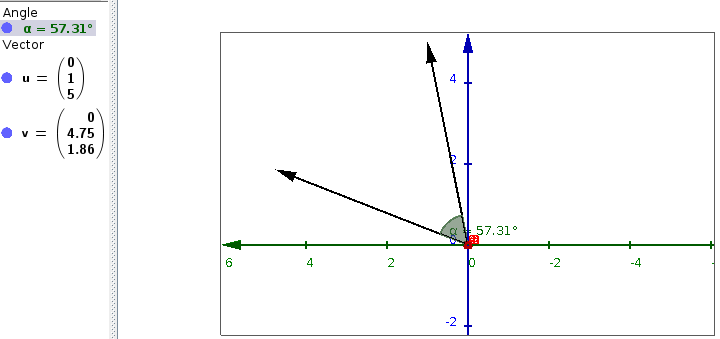
\includegraphics[width=12cm]{rotationsmatrix_eksempel.png}
  \caption{Eksempel på en rotationsmatrix}
  \label{fig:rotationsmatrix_eksempel}
\end{figure}
% Geogebra udregner vinkler i grader, så vi omregner grader til radianer ved hjælp af ligningen:
% \begin{equation}
  % R=d/2*\pi/360=57,31/2*\pi/360\approx1
% \end{equation}
Vi ser at vektor $\vv{u}$ blev drejet $\theta$ radianer, som forventet.
